\documentclass[a4paper, 10.5pt, twoside]{jreport}

% include
\usepackage{gra_yasuda}
\usepackage{lscape}
\usepackage{graphicx}
\usepackage{here}
\usepackage{color}
\usepackage{amsmath}
\usepackage{subfig}
\usepackage{tascmac}
\usepackage{url}
\usepackage{ascmac}
\usepackage{booktabs}
\usepackage{otf}
\usepackage{comment}



%タイトル
\title{心理的効果を用いた人間とエージェントの繰り返し交渉戦略}
\etitle{Repetitive negotiation strategy of human and agent \\ using psychological effect}

%名前
\author{松下 昌悟}
\eauthor{Shogo MATSUSHITA}

%入学年度
\enteryear{2017}
%卒業年度
\graduateyear{2018}

%学籍番号
\studentnumber{17268508}

%提出日
\date{平成30年1月31日}

\begin{document}

%ここで行ピッチを指定
%フォントを変えるとサイズがリセットされてしまうので注意
\setlength{\baselineskip}{8truemm}


%ここから内容

% Chapter 5
\chapter{評価実験}\label{cha:5}

\section{目的と概要}
提案手法の有効性を示すことを目的として人間とエージェントで交渉を行う.
被験者は提案手法の戦略を適用した8つのエージェントにベースラインであるNotNotエージェントを加えた計9種類のエージェントすべてと交渉を行う.
本実験では,提案手法の戦略を適用したエージェントの個人効用が高いほど良い戦略であると評価する.

\section{実験設定}
評価実験では,予備実験と同様に各論点が$0\sim 5$の計6つの選択肢を有する,4つの論点について交渉を行う.
評価実験で用いるドメインは予備実験で用いたドメイン(表\ref{tab:pre_domain})と同一のものである.
各論点の価値は交渉ごとに毎回ランダムで変化し,エージェントと被験者の各論点の価値の関係は予備実験と同様であり,社会的余剰の最大値は70である.
1交渉300秒とし,被験者はチュートリアルとして1回交渉を行なったのちに,各エージェントと5回連続で交渉を行う.
被験者,エージェントは自分にとっての各論点の価値だけを知っており,相手にとっての価値はわからない状態から交渉が開始する.
相手にとっての価値は相手の選好に関する返答や相手の提案内容から予想する.
本実験は9人の被験者に対して行なった.被験者ごとに交渉するエージェントの順番は異なり,ラテン方格法によって決定した.
交渉中,被験者は以下の行動を取ることができる.
\begin{enumerate}
  \renewcommand{\labelenumi}{(\arabic{enumi})}
  \item 自分の選好の相対的な関係を1つ相手に伝える
  \item 相手の選好について質問する
  \item 自分の感情を相手に伝える
  \item 相手に固定メッセージを送信する
  \item エージェントに提案を行う
  \item エージェントから送られてきた提案を受諾もしくは拒否する
  \item 被験者にとっての各論点の価値を確認する
\end{enumerate}
交渉はエージェントと被験者の両者がFullOfferを受諾するか交渉の残り時間が0になると終了する.
基本的にエージェントは被験者の行動に対して受動的に行動する.
例として,被験者が(1)の行動を行うとエージェントは自分の選好の相対的な関係を1つ被験者に伝える.
他の被験者の行動に対しても同様である.
エージェントが被験者に対して能動的に提案を行うのは交渉の残り時間が30秒となったとき,被験者がエージェントに提案を要求する固定メッセージを送信したときだけである.同様にエージェントから新しい提案を行うことはなく,被験者から送信された提案を拒否した場合に提案を行う.
予備実験をもとに戦略ごとに決定したパラメータを表\ref{tab:eva_para}に示す.被験者はこれらのエージェントと交渉を行う.

\begin{table}[tb]
  \begin{center}
    \caption{評価実験で用いるパラメータ}
    \label{tab:eva_para}
    \begin{tabular}{|c|c|c|c|c|c|} \hline
      & \alpha の初期値 & \alpha の増分 & \beta の初期値 & \beta の増分 & \alpha の更新回数 \\ \hline \hline
      NotNot & 0.0 & 0.0 & 0.0 & 0.0 & 0 \\ \hline
      NotFoot & 0.0 & 0.0 & 8.0 & 0.5 & 0 \\ \hline
      NotDoor & 0.0 & 0.0 & 8.0 & 0.5 & 0 \\ \hline
      FootNot & 8.0 & 0.5 & 0.0 & 0.0 & 3 \\ \hline
      FootFoot & 0.0 & 0.5 & 0.0 & 0.5 & 1 \\ \hline
      FootDoor & 8.0 & 2.0 & 0.5 & 1.0 & 3 \\ \hline
      DoorNot & 8.0 & 0.5 & 0.0 & 0.0 & 1 \\ \hline
      DoorFoot & 2.0 & 1.0 & 8.0 & 0.5 & 10 \\ \hline
      DoorDoor & 8.0 & 0.5 & 8.0 & 0.5 & 1 \\ \hline
    \end{tabular}
  \end{center}
\end{table}

\section{実験結果と考察}
エージェントの個人効用の平均値,被験者の個人効用の平均値,エージェントと被験者の個人効用の差分の平均値,エージェントと被験者の社会的余剰の平均値,エージェントの交渉決裂率の平均値をそれぞれ図\ref{fig:res_util_vh}-図\ref{fig:res_broken}に示す\footnote{図\ref{fig:res_util_vh}-図\ref{fig:res_broken}のグラフ中のエラーバーは標準偏差である.}.

\begin{figure}[H]
  \centering
  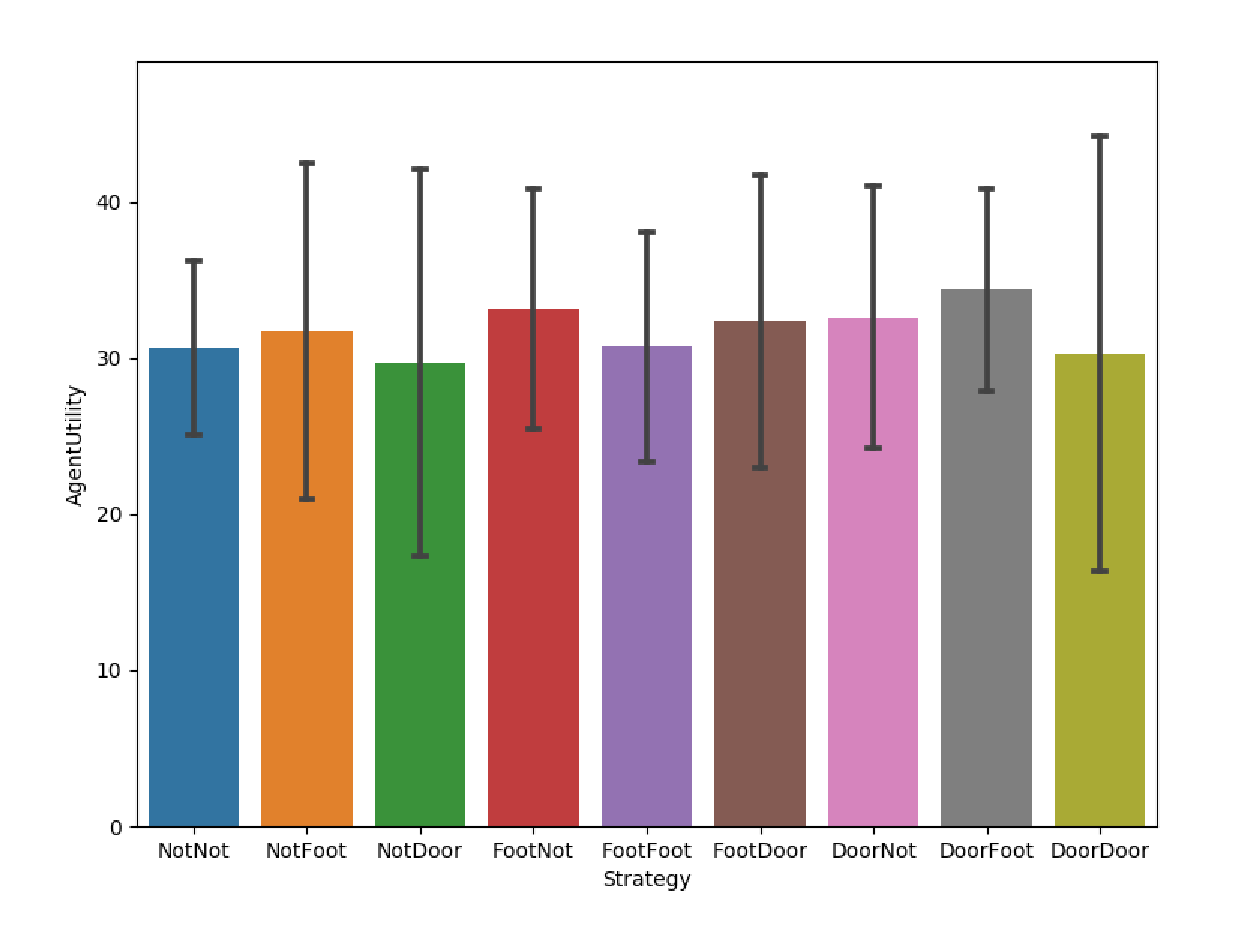
\includegraphics[width=12truecm]{image/util_vh.eps}
  \caption{エージェントの個人効用}
  \label{fig:res_util_vh}
\end{figure}

\begin{figure}[H]
  \centering
  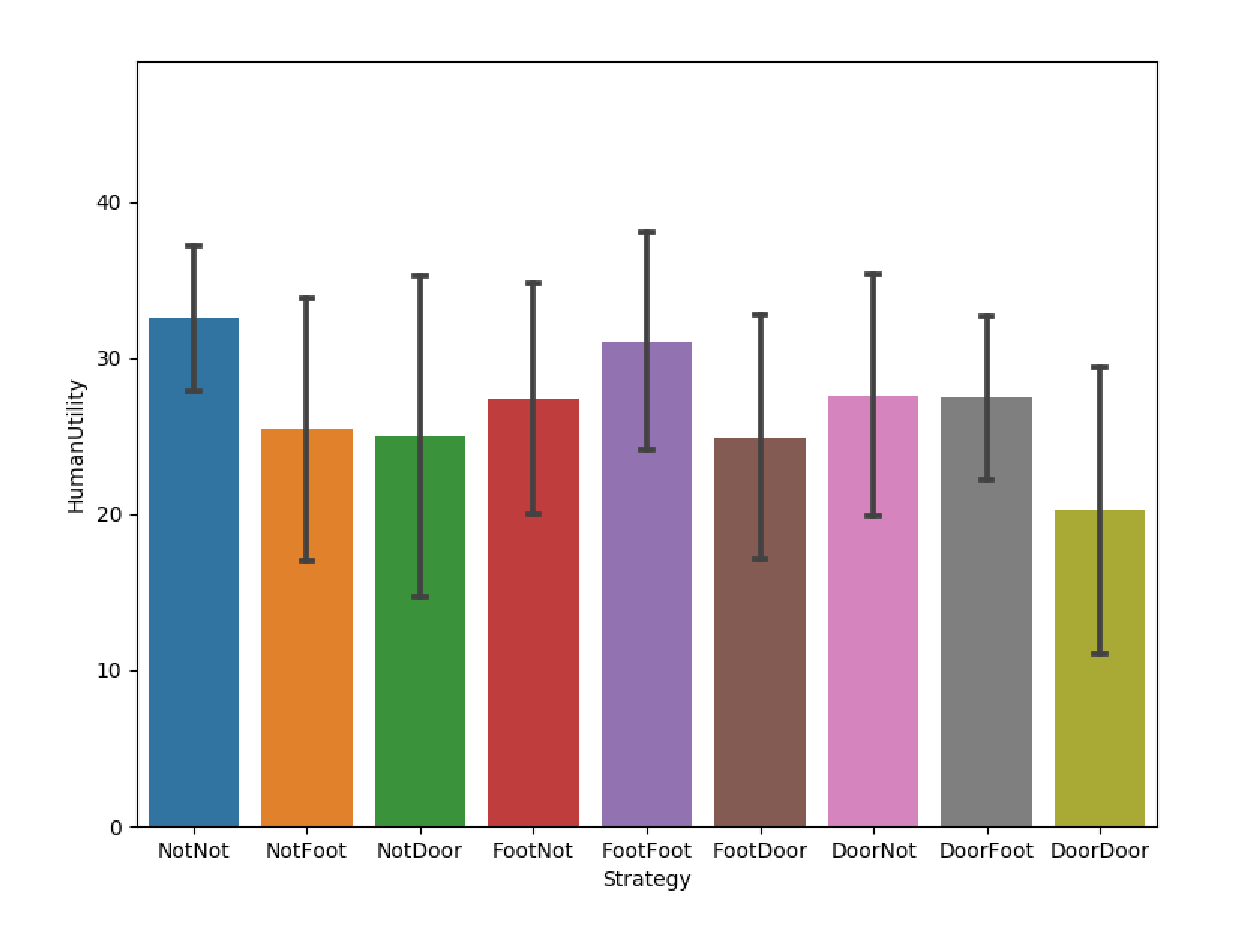
\includegraphics[width=12truecm]{image/util_user.eps}
  \caption{被験者の個人効用}
  \label{fig:res_util_user}
\end{figure}

\begin{figure}[H]
  \centering
  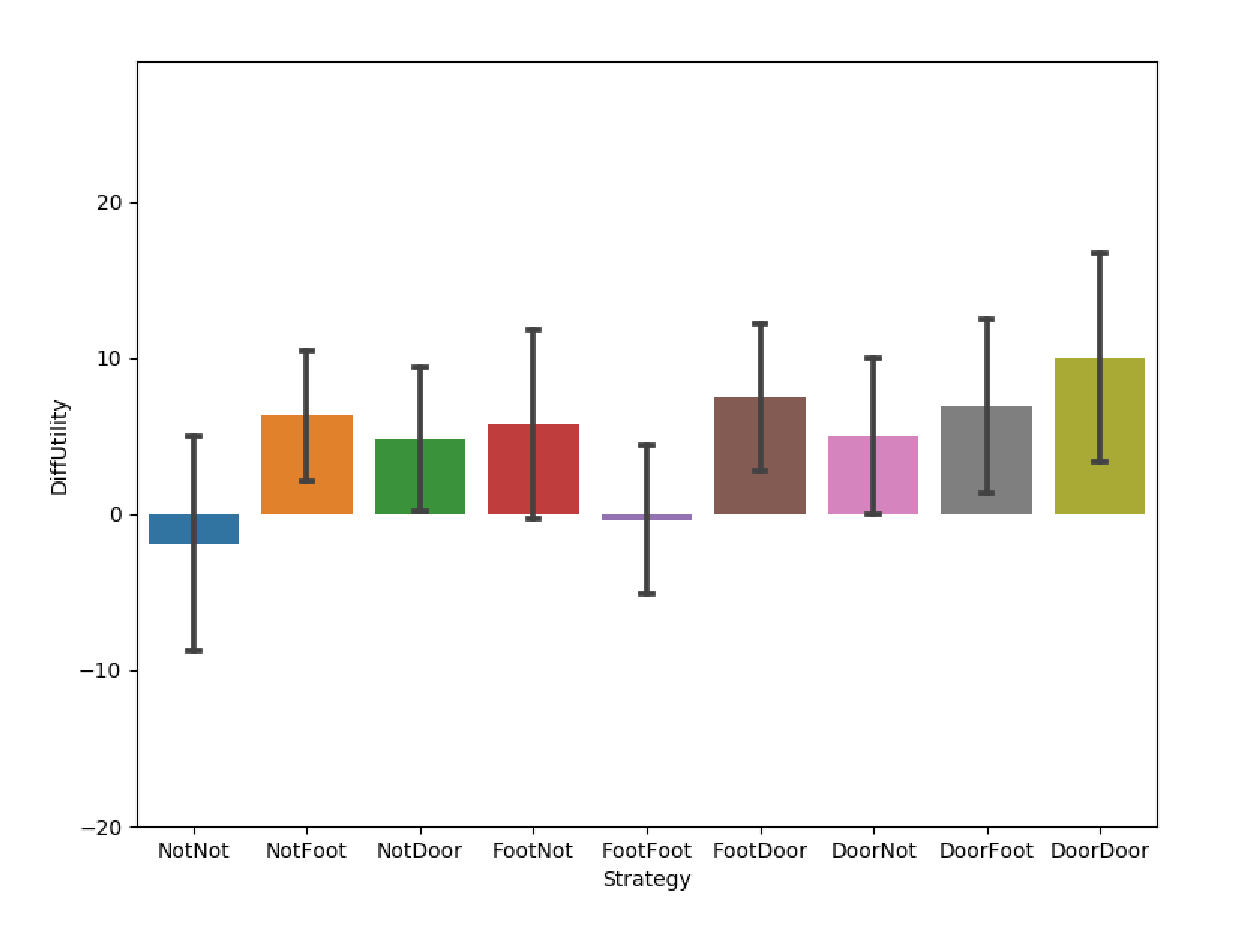
\includegraphics[width=12truecm]{image/result_utility_diff.eps}
  \caption{エージェントと被験者の個人効用の差分}
  \label{fig:res_util_diff}
\end{figure}

\begin{figure}[H]
  \centering
  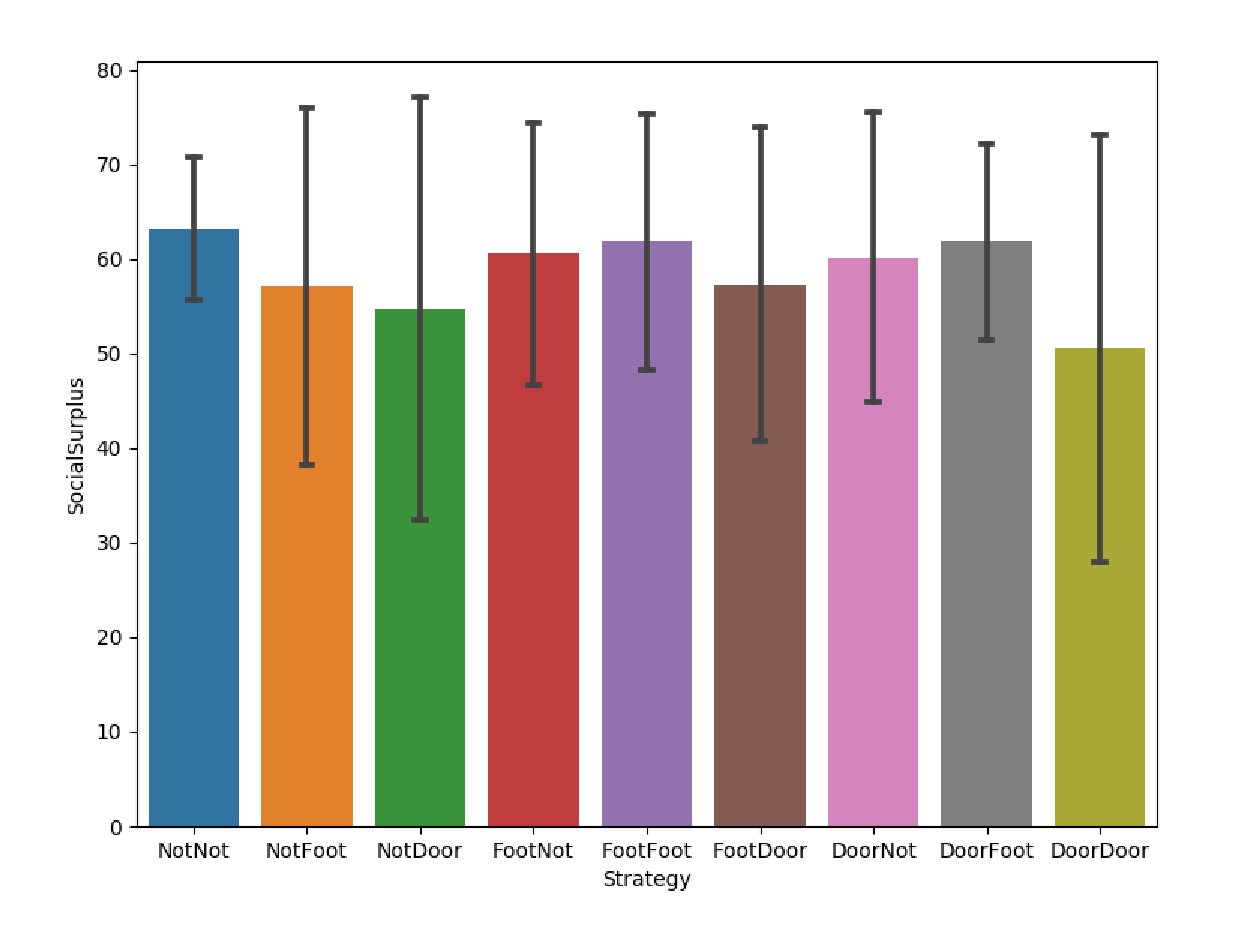
\includegraphics[width=12truecm]{image/result_social_surplus.eps}
  \caption{エージェントと被験者の社会的余剰}
  \label{fig:res_social}
\end{figure}

\begin{figure}[H]
  \centering
  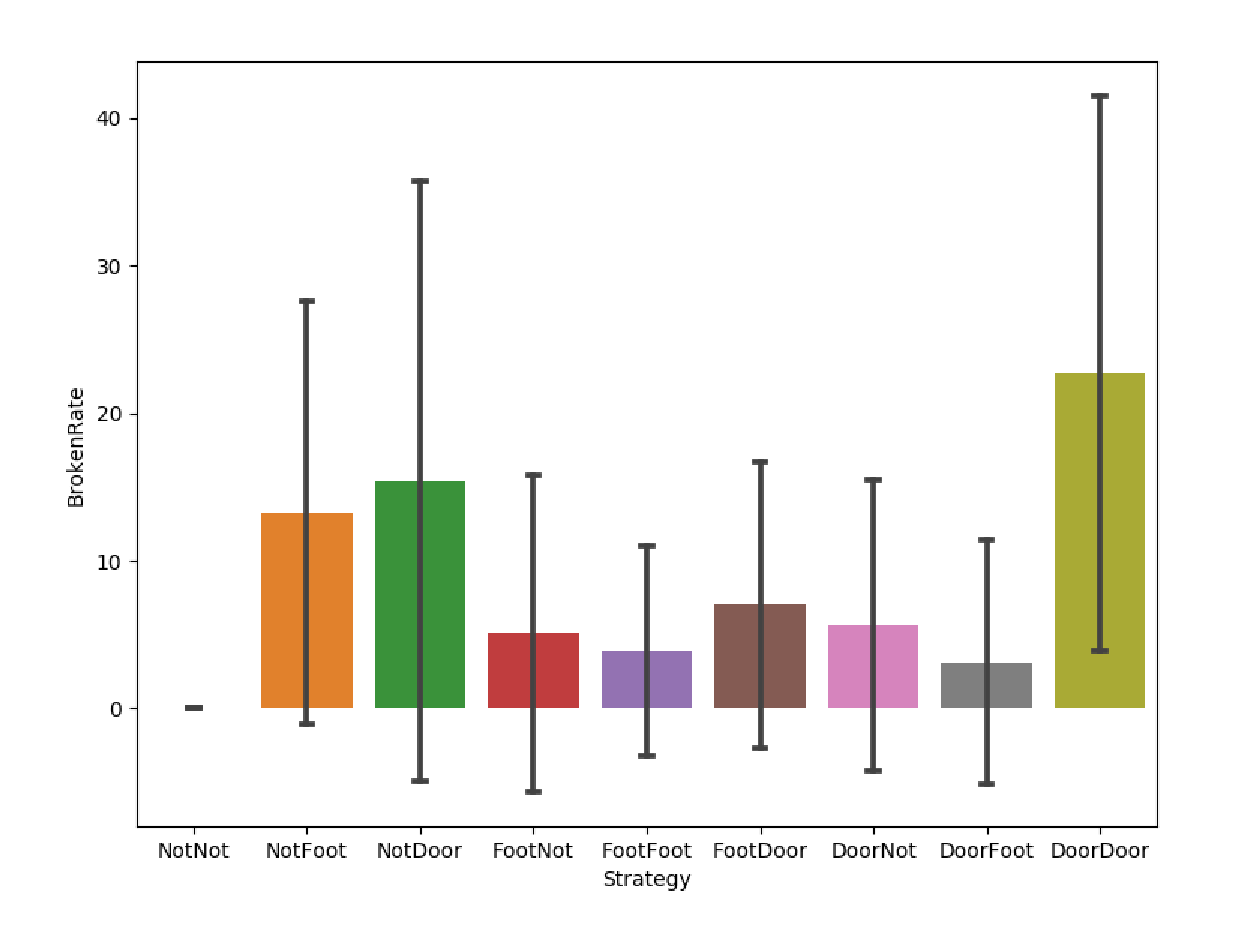
\includegraphics[width=12truecm]{image/result_broken_rate.eps}
  \caption{エージェントの交渉決裂率}
  \label{fig:res_broken}
\end{figure}

各実験結果についてNotNotと提案手法の戦略でそれぞれt検定を行なった.エージェントの個人効用はDoorFootだけが有意差があり,その他の戦略は有意差がない結果になった.被験者の個人効用,エージェントと被験者の個人効用の差分はFootFoot以外は有意差があり,FootFootだけが有意差がない結果になった.
エージェントと被験者の社会的余剰はNotDoor,FootDoor,DoorDoorは有意差があり,それ以外の戦略は有意差がない結果になった.
エージェントの交渉決裂率はDoorDoorだけが有意差があり,DoorDoor以外の戦略は有意差がない結果になった.

NotNot,FootFoot以外の戦略では被験者よりエージェントの方が個人効用が高くなった.
NotNotとFootFootは社会的余剰も高いため,他の戦略と比較するとエージェントと被験者が公平な提案で合意した.今回,FootFootは$\alpha$および$\beta$の増分が小さく.$\alpha$の更新回数も1回であるので,受諾水準がNotNotとあまり変わらなかったためNotNotと類似した結果となった.

DoorDoorは被験者とエージェントの個人効用の差が最大となった.
DoorDoorは$\alpha$および$\beta$の初期値が高く,増分が小さいので受諾水準が高いため,合意に至った場合はエージェントが被験者より個人効用が高くなるが,交渉決裂率も全戦略の中で最も高いため,エージェントおよび被験者の効用,社会的余剰が最も低くなった.

外側にDoorを用いているNotDoor,FootDoor,DoorDoorはいずれも被験者の個人効用が低く,社会的余剰も低くなった.
予備実験におけるDoorの結果を踏まえ,評価実験では$\beta$の初期値を高く,増分を低い値に設定したためエージェントの受諾水準が高くなり,合意に至っても被験者の効用が低くなった.

NotFoot,FootNotは片側にFoot,もう片側にNotを用いた戦略であり,
パラメータの初期値,増分も同じ値であるにも関わらず交渉決裂率の平均がNotFootの方がFootNotと比較して$10\%$程度高くなっている.また,同様にNotDoor,DoorNotも同様の傾向が見られる.このことから,外側戦略の方が被験者に与える影響が大きくなる.

予備実験の結果と比較するとほとんどの戦略で社会的余剰,個人効用ともに減少している.
予備実験ではエージェント同士で交渉を行い,パラメータを設定したため,人間との交渉においては適していないパラメータになっていたため,
個人効用が低下した.また,Doorを用いた戦略は初期値が高く,増分が低いパラメータを設定したため,交渉決裂率が高い戦略が多かった.また,合意に至った場合でも個人効用の差が大きいため,公平な提案で合意が行えておらず,良好な関係構築は果たせていない.9種類のエージェントの中でNotNotだけが唯一交渉決裂率が$0\%$となった.他の戦略はすべてNotNotよりも受諾水準が高いため,これに伴って交渉が決率する回数も多くなった.

\section{実験のまとめ}
評価実験の結果をまとめると以下のようになる.
\begin{itemize}
  \item すべての戦略でNotNotより個人効用の差が大きくなった.
  \item DoorDoor戦略は個人効用の差は最も大きくなったが,社会的余剰,被験者とエージェントの個人効用は最も小さくなった.
  \item 社会的余剰はNotNotよりも低い戦略が多く,良好な関係を構築できているとは言い難い.
\end{itemize}

%内容ここまで

\chapter*{謝辞}
本論文を執筆するにあたり,多数の方々からご指導・ご協力いただきましたことを,心より御礼申し上げます.

指導教員である藤田桂英准教授には,研究の機会を与えていただき,研究の方針に関する助言や発表練習等の
多大なるご指導や助言をいただきましたことを深く感謝いたします.

研究に関する知識のご教示に加えて,本実験の準備を行うにあたってWEBサーバを構築する際にお力添えいただいた松根鷹生様に深く感謝申し上げます.
また,藤田桂英研究室の皆様には研究に必要な知識や意見等をいただいたことを心より感謝いたします.

本実験を行うにあたってお忙しい中ご協力いただいた同期の編入生の方々,および安井貴規様がいなければ本論文は完成に至りませんでした.
心より御礼申し上げます.

最後に,様々な面で私を支えていただいた家族に,心より感謝いたします.ありがとうございました.

\bibliographystyle{plain}
\bibliography{reference}


\begin{comment}
%付録で発表論文をつけてアピールだ!!

\renewcommand{\bibname}{付録 発表論文一覧}
%\chapter{発表論文一覧}

\begin{thebibliography}{99}
\item S. Kakimoto and K. Fujita. 二者間複数論点交渉問題におけるパレートフロント推定手法の提案. Joint Agent Workshop and Symposium, 2014.
\item S. Kakimoto and K. Fujita. Estimating Pareto Fronts using Interdependency between Issues for Bilateral Multi-issue Closed Nonlinear Negotiations. Applications Knowledge and Service Technology for Life, Environment, and Sustainability workshop(KASTLES),2014.
\item S. Kakimoto and K. Fujita. 二者間非線形交渉問題におけるパレートフロント推定を利用した自動交渉エージェントの設計と評価. 情報処理学会 第177回 知能システム研究会, 2014.

\end{thebibliography}

\end{comment}

\end{document}

